\documentclass[12pt]{article}
\usepackage{amsmath}
\usepackage{amssymb}
\usepackage{geometry}
\usepackage{multicol}
\usepackage{parskip}
\usepackage{graphicx}
\setlength{\parindent}{0cm}
\geometry{scale=0.8}
\linespread{1}
%%%
\usepackage{amsfonts,bm}
\usepackage[amsmath,thmmarks,framed]{ntheorem}
\theorembodyfont{\rm}
\theoremstyle{break}
\usepackage{framed}
\usepackage{color}
\definecolor{gray}{rgb}{0.6,0.6,0.6}
\renewcommand*\FrameCommand{{\color{gray}\vrule width 5pt \hspace{10pt}}}
\newframedtheorem{theorem}{Theorem}
\newframedtheorem{algorithm}{Algorithm}
\theoremstyle{nonumberbreak}
\newframedtheorem{definition}{Definition}
\newenvironment{proof}{{\noindent\it Proof}\quad}{\hfill $\square$\par}
%%%
\usepackage{paralist}
\let\itemize\compactitem
\let\enditemize\endcompactitem
\let\enumerate\compactenum
\let\endenumerate\endcompactenum
\let\description\compactdesc
\let\enddescription\endcompactdesc
%%%
\makeatletter 
\renewcommand
\normalsize{   
    \@setfontsize\normalsize\@xpt\@xiipt    
    \abovedisplayskip 4\p@ \@plus2\p@ \@minus5\p@  
    \abovedisplayshortskip \z@ \@plus3\p@    
    \belowdisplayshortskip \p@ \@plus3\p@ \@minus3\p@    
    \belowdisplayskip \abovedisplayskip    
    \let\@listi\@listI} 
\makeatother
%%%
\title{Notes for CIE 6002 Matrix Analysis}
\author{Binghao He}
\date{\today}
\setcounter{secnumdepth}{0}


\begin{document}
\maketitle    
\tableofcontents

\newpage
\section{Lecture 2. Fundamental and Basic Operations}
\begin{multicols}{2}
\subsection{Subspace}
\subsubsection{Definition}
The set $S\subseteq\mathbb{R}^m$ is a subspace, if for $x,y\in S$
\[
    \alpha x + \beta y = S,\quad \alpha, \beta \in \mathbb{R}^m
\]
This indicates
\[
    x_i\in S,\quad i=1,...,N\quad \Longrightarrow\quad \sum_{i=1}^N\alpha_i x_i \in S
\]
\subsubsection{Some important subspaces}
\begin{enumerate}
    \item Span: a collection of vectors 
    \[
        span\{a_1,...,a_n\}=\{y\in\mathbb{R}^m | y= \sum_{i=1}^n\alpha_ia_,\alpha_i\in\mathbb{R}\}
    \]
    \item Orthogonal complement: given a subspace $S\subseteq \mathbb{R}^m$
    \[
        S_\bot = \{y\in\mathbb{R}^m|y^Tx=0,\forall x\in S\}
    \]
    \item Range space of $A$ (linear comb. of col. vectors)
    \[
        \begin{array}{rl}
            R(A) &= span\{a_1,a_2,...,a_n\} \\
            & =\{y\in\mathbb{R}^m|y=Ax,x\in\mathbb{R}^n\}
        \end{array}       
    \]
    \item Null space of $A$ (linear comb. of col. vectors)
    \[
        Null(A)=\{x\in\mathbb{R}^n|Ax=0\}
    \]
\end{enumerate}
\subsubsection{Linear independence}
Given a set $\{a_1,a_2,...,a_n\}$, we say they are linear independent if
\[
    \sum_{i=1}^n\alpha_ia_i=0\Longrightarrow \alpha_i=0,\forall i=1,...,n
\]
\subsubsection{Basis}
$\{b_1,b_2,...,b_k\}\subseteq \mathbb{R}^m$ is a basis for the subspace $S\subseteq \mathbb{R}^m$ 
if $S=span\{b_1,b_2,...,b_k\}$ and $\{b_1,b_2,...,b_k\}$ is linear independent. \\
The number of the vectors of the basis for $S$
\[
    k=dim(S)
\]
\begin{enumerate}
    \item $k$: max number of linear indep. vectors in $S$
    \item $k$: min number of vectors that can span $S$
\end{enumerate}
\subsubsection{Rank}
For a matrix $A\in\mathbb{R}^{m\times n}$
\[
    dim(R(A))\leq min\{m,n\}
\]
Rank of a matrix (?)
\[
    \begin{array}{cll}
        rank(A) & = &dim(R(A)) \\
        & = &\text{\rm max number of linearly indep.} \\
        & & \text{\rm columns(rows) of } A \\
        & = &rank(A^T)
    \end{array}
\]
And
\[
    Null(A)=(R(A^T))_\bot
\]

\subsubsection{Nonsingularity/Invertibility}
A symmetric matrix $A\in\mathbb{R}^{m\times m}$ is non-singular if
\[
    Ax=0\quad \Longrightarrow \quad x=0
\]
$\Longrightarrow$ columns of $A$ are linearly indep. \\
$\Longrightarrow$ $\exists A^{-1}\in\mathbb{R}^{m\times m}$ that $AA^{-1}=A^{-1}A=I_m$ \\
Some properties
\begin{enumerate}
    \item $(AB)^{-1}=B^{-1}A^{-1}$
    \item $(A^{-1})^T=(A^T)^{-1}$
\end{enumerate}

\subsubsection{Determinant}
For a matrix $A\in\mathbb{R}^{m\times m}$, \\
Inductive
\begin{enumerate}
    \item If $m=1$, $det(A)=A$
    \item If $m>1$,
    Define: $A_{ij}\in\mathbb{R}^{(m-1)\times(m-1)}$ is a submatrix that removes $i$th row and 
    $j$th column of $A$. \\
    Define: $c_ij=(-1)^{i+j}det(A_{ij})$. \\
    $\begin{array}{lll}
        det(A) &=\sum_{j=1}^m a_{ij}c_{ij}& \forall i=1,...,m \\
        & = \sum_{i=1}^m a_{ij}c_{ij} & \forall j = 1,...,m
    \end{array}$
\end{enumerate}
For $A,B\in\mathbb{R}^{m\times m}$
\begin{itemize}
    \item [-] $det(AB)=det(A)det(B)$
    \item [-] $det(A)=det(A^T)$
    \item [-] $det(\alpha A)=\alpha^m det(A)$
    \item [-] $det(A)=0$ $\Longleftrightarrow$ $A$ is singular
    \item [-] $det(A^{-1})=1/det(A)$ if $A$ is invertible
\end{itemize}

\subsection{Vector Norm}
A mapping $f:\mathbb{R^m}\to\mathbb{R}$ is a norm if it satisfies that $\forall x,y\in\mathbb{R}^m$
\begin{itemize}
    \item [-] $f(x)\geq 0$
    \item [-] $f(x)= 0$ \emph{iff.} $x=0$
    \item [-] $f(x+y)\leq f(x)+f(y)$
    \item [-] $f(\alpha x)=|\alpha|f(x)$
\end{itemize}
Examples
\begin{itemize}
    \item [-] $\|x\|_2=\sqrt{\sum_{i=1}^m|x_i|^2}$ (Euclidean norm)
    \item [-] $\|x\|_1=\sum_{i=1}^m|x_i|$
    \item [-] $\|x\|_\infty=\max_{i=1,...,m}|x_i|$
    \item [-] $\|x\|_p=\sqrt[p]{\sum_{i=1}^m|x_i|^p}$
\end{itemize}

\subsection{Inner Product}
\[
    <x,y>=x^Ty
\]
\[
    <x,x>=\|x\|_2^2
\]
Cauchy-Schwarz Inequality 
\[
    |x^Ty|\leq \|x\|_2\cdot \|y\|_2
\]
Holder Inequality
\[
    |x^Ty|\leq \|x\|_p\cdot \|y\|_q
\]
where
\[
    1/p+1/q=1\quad ,\quad p\cdot q\geq 1
\]

\subsection{Projection onto a Subspace}
\subsubsection{Projection}
Given a set $S\subseteq \mathbb{R}^m$ and a point $y\in\mathbb{R}^m$, the projection of $y$ onto $S$ is
\[
    y_S=\arg \min_{z\in S} \|z-y\|_2^2
\]
\begin{theorem}
    Suppose $S$ is a subspace,
    \begin{enumerate}
        \item $y_S$ exists and is unique
        \item Let $y_S=\Pi_S(y)$ \emph{iff.} \\
        $z^T(y_S-y)=0$ $\forall z\in S$
    \end{enumerate}    
\end{theorem}

\subsubsection{Orthogonal complement}
$S_\bot =\{y\in\mathbb{R}^m|y^Tx=0,\forall x\in S\}$ is the orthogonal complement 
of subspace $S$. 
\begin{itemize}
    \item [-] Orthogonal complement is a subspace
    \item [-] $S \cap S_\bot$
\end{itemize}
\begin{theorem} \label{th2}
    
    Let $S\subseteq \mathbb{R}^m$ be a subspace. For any $y\in\mathbb{R}^m$
    \[
        y=\Pi_S(y) + \Pi_{S_\bot}(y)
    \]
\end{theorem}
\begin{proof}
    \[
        y=\Pi_S(y) + \Pi_{S_\bot}(y)
    \]
    \[
        \begin{array}{ll}
            \Longleftrightarrow & y-\Pi_S(y)=\Pi_{S_\bot}(y) \\
            \Longleftrightarrow & z^T(y-y+\Pi_S(y))=0 \quad \forall z\in S_\bot \\
            \Longleftrightarrow & z^T\Pi_S(y)=0 \quad \forall z\in S_\bot 
        \end{array}
    \]
    \[
        \because\quad \Pi_S(y))\in S 
    \]
    \[
        \therefore z^T\Pi_S(y))=0 \quad \forall z\in S_\bot 
    \]
\end{proof}

\subsubsection{Sum of subspaces}
For two sets $X,Y\subseteq \mathbb{R}^m$,
\[
    X+Y=\{x+y\in\mathbb{R}^m\}
\]
For a subspace $S\subseteq \mathbb{R}^m$
\begin{enumerate}
    \item $S+S_\bot = \mathbb{R}^m$
    \item $dim(S)+dim(S_\bot)=m$
    \item $(S_\bot)_\bot = S$
\end{enumerate}
\begin{proof}
    \begin{enumerate}
        \item Comes from Theorem \ref{th2}
        \item Let $\{a_1,a_2,...,a_k\}$ be a basis for $S$ ($dim(S)=k$) and $\{b_1,b_2,...,b_\ell\}$ be a basis for $S\bot$ ($dim(S_\bot)=\ell$).
        \\ $\{a_1,a_2,...,a_k\}\cup\{b_1,b_2,...,b_\ell\}$ is 
        \begin{enumerate}
            \item linear independent
            \item Span $S+S_\bot=\mathbb{R}^m$
        \end{enumerate}
        Therefore, $dim(S)+dim(S_\bot)=m$
        \item Obvious
    \end{enumerate}
\end{proof}

\subsubsection{Orthogonal Set}
$\{a_1,a_2,...,a_n\}$ is orthogonal/orthonormal set if
\begin{enumerate}
    \item $\|a_i\|_2=1\quad \forall i=1,...,n$
    \item $a_i^Ta_j= 0\quad \forall i\neq j$
\end{enumerate}
The orthogonal set is linear independent.
\[
    y=\sum_{i=1}^n\alpha_ia_i \Longrightarrow \alpha_i=a_i^Ty=\alpha \|a_i\|_2^2
\]
Given a linear independent set $\{a_1,a_2,...,a_n\}$. The procedure of finding an orthogonal 
set $\{q_1,q_2,...,1_n\}$ so that $span\{a_1,a_2,...,a_n\}=span\{q_1,q_2,...,q_n\}$ is called 
"Gram-Schimit" procedure.

\subsubsection{Orthogonal/Unitary Matrix}
$Q = [q_1,q_2,...,q_m]\in\mathbb{R}^{n\times m}$, $q_i,i=1,...,m$ are orthogonal.
\begin{itemize}
    \item [-] If $m=n$, \\ $Q$ is orthogonal matrix $\Longrightarrow$ $Q^TQ=I_m=QQ^T$.
    \item [-] If $n>m$, \\ semi-orthogonal $\Longrightarrow$ $Q^TQ=I_m\neq QQ^T$.
\end{itemize}
$Q = [q_1,q_2,...,q_m]\in\mathbb{C}^{n\times m}$, $q_i,i=1,...,m$ are orthogonal.
\begin{itemize}
    \item [-] If $m=n$, \\ $Q$ is unitary matrix $\Longrightarrow$ $Q^HQ=I_m=QQ^H$.
    \item [-] If $n>m$, \\ semi-unitary $\Longrightarrow$ $Q^HQ=I_m\neq QQ^H$.
\end{itemize}
If $Q\in\mathbb{R}^{n\times m}$ $(n>m)$ is semi-orthogonal, $\exists\tilde{Q}\in\mathbb{R}^{n\times(n-m)}$ so that 
$\left[\begin{array}{cc}Q&\tilde{Q}\end{array}\right]$ is orthogonal.
\subsubsection{Dimensional Theorem}
For a matrix $A\in\mathbb{R}^{m\times n}$, it holds
\[
    dim(R(A))+dim(Null(A))=n
\]
\begin{proof}
    \[
        dim(R(A^T))+dim(R(A^T)_\bot)=n
    \]
    \[
        dim(R(A^T))=rank(A^T)=rank(A)=dim(R(A))
    \]
    \[
        dim(R(A^T)_\bot)=Null(A)=n
    \]
\end{proof}

\subsection{Complexity of Matrix Computation}
\subsubsection{Flops}
Arithmetic operations including addition, substraction, multiplication, division.

\subsubsection{Big O notation}
Big O notation: "order" of the complexity.
\[
    f(n)=O(g(n))
\] 
for some $g(n)$ if $\exists$ a constant $C>0$ and $n_0$ so that for $n>n_0$
\[
    |f(n)|\leq C\cdot|g(n)|
\]
Examples: for $x\in\mathbb{R}^m$, $y\in\mathbb{R}^m$, $A\in\mathbb{R}^{n\times m}$, $B\in\mathbb{R}^{m \times p}$
\[
    \begin{array}{ccl}
        x+y & m \text{ \rm flops} & O(m) \\
        x^Ty& 2m-1 \text{ \rm flops}  & O(m) \\
        Ax  & n\cdot(2m-1) \text{ \rm flops} & O(nm) \\ 
        AB  & p\cdot n \cdot (2m-1)\text{ \rm flops} & O(pnm) \\ 
    \end{array}
\]
\newpage    
\end{multicols}


\section{Lecture 3. Least Square Problem (LSP)}
\begin{multicols}{2}
\subsection{Formulation}
\subsubsection{LS problem}
Given $y\in\mathbb{R}^m$, $A\in\mathbb{R}^{m\times n}$
\[
    \min_{x\in\mathbb{R}^n} \|y-Ax\|_2^2
\]
\subsubsection{Linear representation of signals}
\[
    y=Ax
\]
In practice,
\[
    y=Ax+v
\]
where 
\begin{itemize}
    \item [-] $y$ is the observation (Given)
    \item [-] $A$ is the model (Given)
    \item [-] $x$ is the parameter to be estimated/determined
    \item [-] $v$ is the noice follow multi-variate Gaussian distribution
    \[
        \text{\rm pdf}(v)\propto e^{-\|v\|^2}
    \]
\end{itemize}
$\Longrightarrow$ Maximum likelihood estimator 
\[
    \max_x P(y|x) \propto \min_x \|y-Ax\|_2^2
\]
\subsection{AR and Polynomial Models}
\subsubsection{Autoregressive (AR) model}
Given  a time series $y_t$, $t=0,1,2,...$, 
\[
    \underbrace{y_t = \alpha_1y_{t-1} + \alpha_2y_{t-2} +\cdots +\alpha_py_{t-p}}_{\text{\rm AR model}} + \underbrace{v_t}_{\text{\rm noise}}
\]
If $\alpha_1,\alpha_2,...,\alpha_p$ are known, estimate $y_t$ by 
\[
    \hat{y}_t =  \underbrace{\alpha_1y_{t-1} + \alpha_2y_{t-2} +\cdots +\alpha_py_{t-p}}_{\text{\rm historical observation}}
\]
Collect
\[
    \underbrace{
    \left[\begin{array}{l}
        y_0 \\
        y_1 \\
        \vdots \\
        y_T
    \end{array}
    \right]}_{y\in\mathbb{R}^T}
    =
    \underbrace{
    \left[\begin{array}{cccc}
        y_0 &     & &\\
        y_1 & y_0 && \\
        \vdots & \ddots& \ddots & \\
        y_{p-1}& \cdots& \cdots & y_0 \\
        \vdots &  \ddots&\ddots & \vdots \\
        y_{T-1} & \cdots&\cdots & y_T
    \end{array}
    \right]}_{A\in\mathbb{R}^{T\times p}}
    \underbrace{
    \left[\begin{array}{l}
        \alpha_1 \\
        \alpha_2 \\
        \vdots \\
        \alpha_p
    \end{array}
    \right]}_{x\in\mathbb{R}^p}
    +
    \underbrace{
    \left[\begin{array}{l}
        v_0 \\
        v_1 \\
        \vdots \\
        v_T
    \end{array}
    \right]}_{v\in \mathbb{R}^T}
\]
$\Longrightarrow$ Solve LS problem to obtain $\alpha_i$, $i=1,...,p$
\subsubsection{Polynomial model}
\[
    \underbrace{y_t = \alpha_0 + \alpha_1t + \alpha_2t^2 +\cdots +\alpha_pt^p}_{\text{\rm polynomial model}} + \underbrace{v_t}_{\text{\rm noise}}
\]
Collect
\[
    \underbrace{
    \left[\begin{array}{l}
        y_0 \\
        y_1 \\
        \vdots \\
        y_T
    \end{array}
    \right]}_{y\in\mathbb{R}^T}
    =
    \underbrace{
    \left[\begin{array}{cccc}
        1 & 0  & \cdots & 0 \\
        1 & 1  & \cdots & 1 \\
          &   \vdots &   &   \\
        1 & t  & \cdots & t^p \\
          &    \vdots &   &   \\
        1 & T-1  & \cdots & (T-1)^p
    \end{array}
    \right]}_{A\in\mathbb{R}^{T\times p}}
    \underbrace{
    \left[\begin{array}{l}
        \alpha_1 \\
        \alpha_2 \\
        \vdots \\
        \alpha_p
    \end{array}
    \right]}_{x\in\mathbb{R}^p}
    +
    \underbrace{
    \left[\begin{array}{l}
        v_0 \\
        v_1 \\
        \vdots \\
        v_T
    \end{array}
    \right]}_{v\in \mathbb{R}^T}
\]
$\Longrightarrow$ Solve LS problem to obtain $\alpha_i$, $i=1,...,p$
\subsection{Basis Representation}
\subsubsection{Basis matrix}
For $y\in\mathbb{R}^m$, given a set of basis vectors (can be given or learned)
\[
    \Phi =\{\phi _1,\phi _2,...,\phi _n\}\in\mathbb{R}^{m\times n}
\]
We model 
\[
    y=\sum_{i=1}^n\phi_ix_i = \Phi x
\]
\begin{enumerate}
    \item [-] $m\gg n$, assume data lies in a low-dimensional subspace 
    \item [-] $m\ll n$, dictionary $\Longrightarrow$ $x$ is sparse
\end{enumerate}
\subsubsection{Fourier basis}
Discrete Fourier Transform (DFT) \\
Inverse Discrete Fourier Transform (IDFT)
\[
    \Phi = [\phi_1,...,\phi_n]\in\mathbb{C}^{n\times n}
\]
\[
    \phi_i = \frac{1}{\sqrt{n}}
    \left[\begin{array}{l}
        1 \\
        e^{j\frac{2\pi}{n}(i-1)} \\
        e^{j\frac{2\pi}{n}(i-1)\times 2} \\
        \vdots \\
        e^{j\frac{2\pi}{n}(i-1)\times {n-1}}
    \end{array}
    \right]
    \in\mathbb{R}^{n} \quad
\]
\begin{itemize}
    \item [-] $\Phi$ is IDFT matrix, $\Phi^H$ is DFT matrix.
    \item [-] $\Phi$ is unitary matrix.
\end{itemize}

\subsection{LTI System}
\subsubsection{Lienar time invariant system}
\[
    \begin{array}{ll}
        -\text{ \rm Linearity} & 
        \left\{\begin{array}{c}
            x_t^1\to \boxed{\text{\rm LTI}} \to y_t^1 \\
            x_t^2 \to \boxed{\text{\rm LTI}} \to y_t^2 \\
            \alpha x_t^1 + \beta x_t^2\to \boxed{\text{\rm LTI}} \to \alpha y_t^1 +\beta y_t^2
        \end{array}
        \right.
        \\
        -\text{ \rm Time Invariant} & x_{t-d}\to \boxed{\text{\rm LTI}} \to y_{t-d}
    \end{array}
\]
Impulse $\delta(t)$
\[
    \left\{\begin{array}{l}
        \delta(t)=0,t\neq 0 \\
        \int_{-\infty}^{+\infty}\delta(t) \,dt 
    \end{array}\right.
\]
LTI system is characterized by an impulse response 
\[
    h_t,\quad t=0,...,p-1
\]
$\Longrightarrow$ $x_t$ and $y_t$ is related through "convolution"
\[
    \begin{array}{ll}
        y_t&=\sum_{i=1}^p {h_i x_{t-i}} \\
        &=h_t\ast x_t
    \end{array}
\]
\[
    x_t\to\overbrace{\boxed{h_t}}^{\text{\rm LTI}}\to y_t
\]
\subsubsection{System identification}
Given $\{y_t\}_{t=0}^{T-1}$ and $\{x_t\}_{t=0}^{T-1}$, find the impulse response $\{h_t\}_{t=0}^{p}$
\[
    \left[\begin{array}{l}
        y_0 \\
        y_1 \\
        \vdots \\
        y_p \\
        \vdots \\
        y_T
    \end{array}
    \right]
    =
    \left[\begin{array}{cccc}
        x_0 &     & &\\
        x_1 & x_0 && \\
        \vdots & \ddots& \ddots & \\
        x_p& \cdots& \cdots & x_0 \\
        \vdots &  \ddots&\ddots & \vdots \\
        x_{T-1} & \cdots&\cdots & x_{T-p}
    \end{array}
    \right]
    \left[\begin{array}{l}
        h_0 \\
        h_1 \\
        \vdots \\
        h_p
    \end{array}
    \right]
    +
    \text{ \rm noise}
\]
$\Longrightarrow$ Solve LS problem to obtain $\{h_t\}_{t=0}^{p}$
\subsubsection{Deconvolution}
Given $\{y_t\}_{t=0}^{T-1}$ and ${h_t}_{t=0}^p$, find out $\{x_t\}_{t=0}^{T-1}$ \\
Put them into a linear system of equations
\[
    \left[\begin{array}{l}
        y_0 \\
        y_1 \\
        \vdots \\
        y_p \\
        \vdots \\
        y_T
    \end{array}
    \right]
    =
    \underbrace{
    \begin{bmatrix}
        h_0   & 0       &         & \cdots  &        &        &  0              \\  
        h_1   & h_0     &    0    & \cdots  &        & \ddots &                \\
        \vdots& \vdots  &         & \ddots  &        &        & \vdots         \\
        h_p   & h_{p-1} &         & \cdots  &        &h_1     & h_0            \\
        \vdots& \ddots  & \ddots  &         &        & \vdots & \vdots         \\
        0     & \cdots  & h_p     & h_{p-1} &\cdots  & h_1    & h_0
    \end{bmatrix}}_{A\in\mathbb{R}^{T\times T}}
    \left[\begin{array}{l}
        x_0 \\
        x_1 \\
        \vdots \\
        x_p \\
        \vdots \\
        x_T
    \end{array}
    \right]
    +
    \text{ \rm noise}
\]
$\Longrightarrow$ Solve LS problem to obtain $\{x_t\}_{t=0}^{T-1}$
\subsubsection{Toeplitz matrix}
\[
    A = 
    \begin{bmatrix}
        a_{0}  & a_{-1}& \cdots & \cdots & a_{-n+1}    \\
        a_{1}  & a_{0} & a_{-1} & \cdots & a_{-n+2}    \\
        a_{2}  & a_{1} & a_{0}  & a_{-1} & \ddots       \\
        \vdots & \ddots&\ddots  & \ddots & \vdots       \\
        a_{n-1}& \cdots&a_{2}   & a_{1}  & a_{0}
    \end{bmatrix}
    \in\mathbb{R}^{n\times n}
\]
\subsection{Circulant Matrix}
Circulant matrix is a special case of Toeplitz matrix
\[
    H = 
    \begin{bmatrix}
        h_{0}  & h_{n-1} & \cdots  & \cdots  & h_{1}    \\
        h_{1}  & h_{0}   & h_{n-1} & \cdots  & h_{2}    \\
        h_{2}  & h_{1}   & h_{0}   & h_{n-1} & \ddots       \\
        \vdots & \ddots  &\ddots   & \ddots  & \vdots       \\
        h_{n-1}& \cdots  &h_{2}    & h_{1}   & h_{0}
    \end{bmatrix}
    \in\mathbb{R}^{n\times n}
\]
\[
    H\overbrace{\Longrightarrow}^{O(n\log n)} H^{-1}
\]
The key property:
\[
    H\cdot \underbrace{\phi_i}_{\text{\rm IDFT}} = d_i\cdot \phi_i\quad , d_i\in\mathbb{R}
\]
Let 
\[
    D = \begin{bmatrix}
        d_1 && \\
        & \ddots & \\
        && d_n 
    \end{bmatrix}
\]
Then 
\[
    \begin{array}{ll}
        H\cdot\Phi &= H\cdot [\phi_1,...,\phi_n]\\
                   &= [d_1\phi_1,...,d_n\phi_n] \\
                   &= \Phi\cdot D
    \end{array}
\]
$\Longrightarrow$
\[
    \underbrace{H = \Phi\cdot D \cdot \Phi^H}_{\text{\rm eigen-decomposition of } H} \Longleftrightarrow \quad \Phi^H H \Phi = D
\]
\newpage
\end{multicols}


\section{Lecture 4. Eigenvalues and Eigenvectors}
\begin{multicols}{2}
\subsection{Definition}
\begin{definition}[Eigenvalues and Eigenvector]
    Let $A\in\mathbb{R}^{m\times m}$, if a scalar $\lambda\in\mathbb{C}$ and a nonzero vector $v\in\mathbb{C}^m$ statisfy the equation 
    \[
        Av=\lambda v
    \]
    then $\lambda$ is called the eigenvalue of $A$ and $v$ is called the eigenvector of $A$ associated with $\lambda$.
\end{definition}
$\Longrightarrow$ 
\[
    \underbrace{(A-\lambda I)}_{\text{\rm singular}}v = 0
\]
The equation $P_A(\lambda)\triangleq det(A-\lambda I)=0$ is called the characteristic euqation of $A$. 
$P_A(\lambda)\triangleq det(A-\lambda I)=\prod_{i=1}^m(\lambda-\lambda_i)$ is a polynomial of $\lambda$ with degree $m$.\\

For each $\lambda$

\newpage
\end{multicols}
\section{Lecture 5. PageRank}
\begin{multicols}{2}
\subsection{PageRank Model}
\subsubsection{Importance score}
\begin{itemize}
    \item [-] $v_i$: importance score of page $i$
    \item [-] $c_j$: number of outgoing links of page $j$
    \item [-] $\mathcal{L}_i$: set of pages that refers to page $i$
\end{itemize}
\[
    \begin{array}{c}
        v_i = |\mathcal{L}_i| \\
        \Downarrow \\
        v_i = \sum_{j\in \mathcal{L}_i} v_j \\
        \Downarrow \\
        v_i = \sum_{j\in \mathcal{L}_i} \frac{v_j}{c_j}
    \end{array}
\]
\subsubsection{The model}
e.g. \\
\centerline{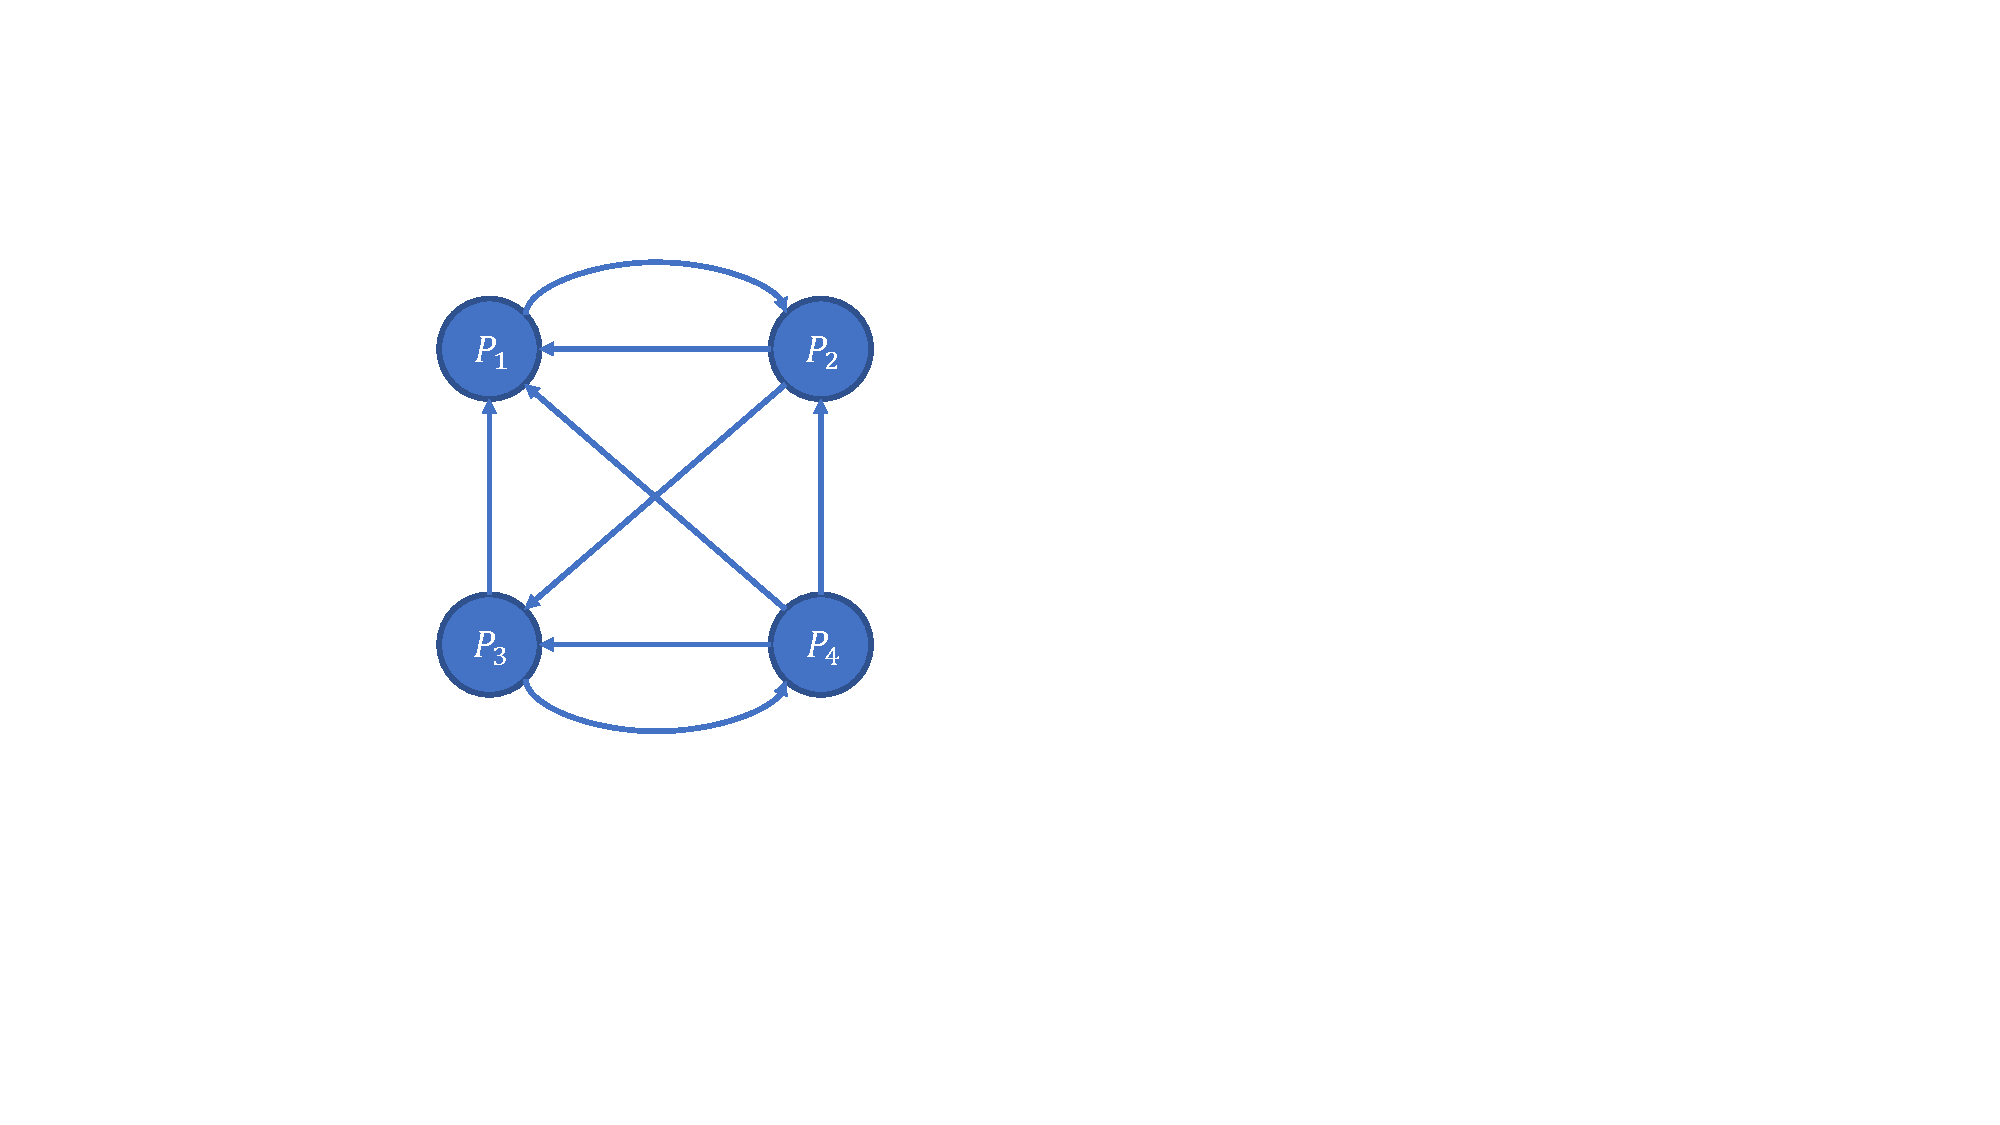
\includegraphics[width=5cm]{sections/lecture_5_fig1.pdf}} \\
$v_1 = 1\cdot v_2 + \frac{1}{2}v_3 + \frac{1}{3}v_4$ \\
$v_2 = 1\cdot v_1 + \frac{1}{3}v_4$ \\
... \\
$\Longrightarrow$
\[
    \underbrace{
    \begin{bmatrix}
        0  &  1/2  &  1/2  &  1/3  \\
        1  &  0    &  0    &  1/3  \\
        0  &  1/2  &  0    &  1/3  \\
        0  &  0    &  1/2  &  0    \\
    \end{bmatrix}
    }_{\text{\rm link matrix}}
    \begin{bmatrix}
        v_1 \\ v_2 \\ v_3 \\ v_4
    \end{bmatrix}
    =
    \begin{bmatrix}
        v_1 \\ v_2 \\ v_3 \\ v_4
    \end{bmatrix}
\]
$\Longrightarrow$
\[
    Av = v\quad ,\quad v \geq 0
\]

\subsection{PageRank Problem}
Find solution $v\geq 0$ satisfying $Av=v$ \\
The foure questions:
\begin{enumerate}
    \item Does $A$ admit a solution of $Av=v$?          \\ (Does $A$ has eigenvalue equal to 1?)
    \item Does $Av=v$ admit a non-negative solution?    \\ ($v\geq 0$ or $v\leq 0$)
    \item Is the solution unique?                       \\ (unique ranking)
    \item Can we obtain the solution efficiently?       \\ (Power method applicable?)
\end{enumerate}

\subsubsection{Answer to Question 1}
Does $A$ admit a solution of $Av=v$? (Does $A$ has eigenvalue equal to 1?)

Note that $A\geq 0$ and column-sum eqaul to 1 (column-stochastic matrix). \\
$\Longrightarrow$ $\textbf{1}^TA=\textbf{1}^T$ \\
$\Longrightarrow$ $A^T\cdot \textbf{1} = \textbf{1}$ \\
$\Longrightarrow$ $A^T$ has an eigenvalue equal to 1 \\
Since $A$ and $A^T$ have the same set of eigenvalues \\
$\Longrightarrow$ $A$ has an eigenvlue equal to 1 \\

\begin{theorem}
    Let $A$ be non-negative and column(row)-stochastic, then
    \begin{enumerate}
        \item $\lambda=1$ is an eigenvlue of $A$
        \item $|\lambda|\leq 1$ for all eigenvalues of $A$
    \end{enumerate}
\end{theorem}
\begin{proof}
    Let $Av = \lambda v$ for some $|\lambda|\neq 1$. \\
    Let $|v_k| = \max \{|v_1|,|v_2|,...,|v_m|\}$.
    \[
        \lambda v_k = \sum_{i=1}^m [A]_{ki}v_i
    \]
    $\Longrightarrow$
    \[
        \begin{array}{ll}
            |\lambda||v_k|  &= |\sum_{i=1}^m[A]_{ki}v_i| \\
                            &\leq \sum_{i=1}^m|[A]_{ki}|\cdot |v_i| \\
                            &\leq |v_k|\cdot \sum_{i=1}^m|[A]_{ki}| \\
                            &= |v_k|
        \end{array}
    \]
    $\Longrightarrow$
    \[
        |\lambda|\leq 1
    \]
\end{proof}

\textbf{Disjoint page networks}
\[
    A = \begin{bmatrix}
        A_1 & 0 \\ 0 & A_2
    \end{bmatrix}
\]
\[
    \begin{array}{l}
        A_1 v_1 = v_1 \\ A_2 v_2 = v_2
    \end{array}
\]
\[
    A
    \left( \alpha_1 \left(\begin{array}{c} v_1 \\ 0 \end{array}\right) + \alpha_2 \left(\begin{array}{c} v_1 \\ 0 \end{array}\right) \right) 
    = 
    \left( \alpha_1 \left(\begin{array}{c} v_1 \\ 0 \end{array}\right) + \alpha_2 \left(\begin{array}{c} v_1 \\ 0 \end{array}\right) \right) 
\]

\textbf{Modified model}
\[
    M \triangleq (1-\beta) A + \beta \left( \frac{11^T}{m} \right) > 0
\]
This is positive column-stochastic
\[
    1^TM = (1-\beta)1^TA + \beta 1^T \left( \frac{11^T}{m} \right) = 1^T
\]

\subsubsection{Answer to Question 2}
Does $Av=v$ admit a non-negative solution? ($v\geq 0$ or $v\leq 0$)

\begin{theorem}
    For positive and column-stochastic matrix $M$, any eigenvector associated with $\lambda_1$ has either all positive or all negative components.
\end{theorem}
\begin{proof}
    Note that for $y\in\mathbb{R}^m$, $|\sum_{i=1}^m y_i| < \sum_{i=1}^m |y_i|$ if $\{y_i\}$ have mixed signs. \\
    Suppose the above theorem is not true. Then we have
    \[
        |v_i| = |\sum_{j=1}^m [M]_{ij}v_j| < \sum_{j=1}^m [M]_{ij}|v_j|
    \]
    $\Longrightarrow$
    \[
        \sum_{i=1}^m |v_i| < \sum_{i=1}^m \sum_{j=1}^m [M]_{ij}v_j = \sum_{j=1}^m\sum_{i=1}^m  [M]_{ij}v_j = \sum_{j=1}^m |v_j|
    \]
    Contradict! So the above theorem is true.
\end{proof}

\subsubsection{Answer to Question 3}
Is the solution unique? (unique ranking) \\
Since $Mv=v$ $\Longrightarrow$ $(M-I)v=0$, show 
\[
    dim(Null(M-I))=1
\]
i.e., there is a unique ranking.

\begin{proof}

    Simple lemma: Let $a$ and $b$ be linearly independent, then $\exists x\in span\{a,b\}$ which has mixed sign. \\
    \emph{Proof for this lemma}: \\
    If $1^Tq=0$ $\Longrightarrow$ $q$ has mixed sign. \\
    If $1^Tq\neq 0$, set $\alpha_1 = \frac{-1^Tb}{1^Tq}$, $\alpha_2=1$ and let $x=\alpha_1\cdot a+\alpha_2\cdot b$ \\
    $\Longrightarrow$ $x$ satisfies $1^Tx=0$, so $x$ has mixed sign.

    Suppose $dim(Null(M-I))>1$, then for $q_1,q_2\in Null(M-I)$ that are linear independent.
    $\Longrightarrow$ $\exists v= \alpha_1 q_1  + \alpha_2 q_2 \in Null(M-I)$ \\
    $\Longrightarrow$ $Mv=v$ which has mixed sign. (Contradict!) \\
    $\Longrightarrow$ $dim(Null(M-I))=1$
\end{proof}

\subsubsection{Answer to Question 4}
Can we obtain the solution efficiently? (Power method applicable?) \\
Property:
Let $M$ be positive and column-stochastic. \\
Let $S=\{v\in \mathbb{R}^m | 1^Tv=0 \}$. \\
Then,
\begin{enumerate}
    \item $Mv\in S$ if $v\in S$
    \item $\|Mv\|_1 \leq c\|v\|_1$ with $c<1$ $\forall$ any $v\in S$
    \item the eigenvector associated with $\lambda=1$, denoted $v_1$, can be obtainable by the power method
\end{enumerate}
\begin{proof} \\
    1) $v\in S$ $\Longleftrightarrow$ $1^Tv=0$ \\
    2) 
\end{proof}
\newpage
\end{multicols}
\section{Lecture 6. Positive Semidefinite Matrix}
\setcounter{theorem}{0}
\begin{multicols}{2}
For $A\in\mathbb{C}^{m\times m}$, if
\begin{itemize}
    \item [-] $A$ is symmetric, we denote $A\in S^m$
    \item [-] $A$ is Hermitian, we denote $A\in H^m$
\end{itemize}
\begin{definition}
    We say $A\in H^m$ is positive semidefinite (PSD) if 
    \[
        x^H A x \geq 0 \quad \forall x\in\mathbb{C}^m
    \]
    We say $A\in H^m$ is positive definite (PD) if 
    \[
        x^H A x > 0 \quad \forall x\in\mathbb{C}^m,x\neq 0
    \]
    We say $A\in H^m$ is indefinite if $A$ is not PSD.
\end{definition}
\subsection{Properties of PSD Matrices}
\subsubsection{Propeties}
\textbf{Property 1}: If $A$ is PSD then any principal submatrix of $A$ ($A_I$) is PSD. \\
\begin{proof} \\
    Let $x\in\mathbb{C}^m$ with $x_{i_k}\neq 0$ for all $i_k \notin I$. \\
    Let $(x_I)_k=x_{i_k}$ for $i_k\in I$. \\
    Then
    \[
        x^HAx = x_I^HA_Ix_I \geq 0,\quad \forall x_I\in \mathbb{C}^{|I|}
    \]
\end{proof}
By Property 1, we know \\
1) 
\[
    A = \begin{bmatrix}
        A_{11} & A_{12} \\ A_{21} & A_{22}
    \end{bmatrix}
\]
\[
    A_{11}\in H^{k\times k}, A_{22}\in H^{(m-k)\times (m-k)}
\]
If $A$ is PSD(PD) $\Longrightarrow$ $A_{11}$, $A_{22}$ are PSD(PD).
2) \\
If $A$ is PSD(PD), then $A_{ii}\geq 0(>0)$

\subsubsection{Eigenvalues of PSD matrices}
\begin{theorem}
    $A\in H^m$ is PSD(PD) if and only if $\lambda_1,\lambda_2,...,\lambda_3\geq 0(>0)$
\end{theorem}
\begin{proof} \\
    Consider EVD of $A$ as 
    \[
        A=V\Lambda V^H, \quad \Lambda=diag(\lambda_1,\lambda_2,...,\lambda_m)
    \]
    Consider $x^HAx=x^HV\Lambda V^Hx=z^H\Lambda z$. 

    $A$ is PSD $\Longleftrightarrow$ $x^HAx\geq 0$ $\forall x\in\mathbb{C}^m$ $\Longleftrightarrow$ $z^H\Lambda z\geq 0$ $\forall z\in\mathbb{C}^m$.

    $z^H\Lambda z=\sum_{i=1}^m \lambda_i |z_i|^2 \geq 0$ $\forall z\in\mathbb{C}^m$ $\Longleftrightarrow$ $\lambda_i\geq 0$ $\forall i=1,...,m$
\end{proof}

If $A$ is PSD(PD),
\begin{itemize}
    \item [-] $Tr(A)\geq 0 (>0)$
    \item [-] $det(A) \geq 0 (>0)$
\end{itemize}

If $A$ is PD, then $A$ is invertible.
\[
    A = V\Lambda V^H
\]
\[
    A^{-1} = V\Lambda^{-1} V^H
\]

\textbf{Property 2}: $A\in H^m$ can be factorized as $A=BB^H$ for some matrix $B$ if and only if $A$ is PSD. \\
\begin{proof} \\
    $\Longrightarrow$:
    \[
        x^HAx = x^HBB^Hx = \|B^Hx\|^2 \geq 0 \Longrightarrow A \text{\rm is PSD}
    \]
    $\Longleftarrow$:\\
    If $A$ is PSD, define $\Lambda^{1/2}=diag(\sqrt{\lambda_1},\sqrt{\lambda_2},...,\sqrt{\lambda_m})$
    \[
        \begin{array}{ll}
            A &= V\lambda V^H \\
            &= V\Lambda^{1/2}\Lambda^{1/2}V^H \\
            &= V\Lambda^{1/2}Q^HQ\Lambda^{1/2}V^H
        \end{array}
    \]
    where $Q$ is a Hermitian matrix. \\
    Define $B\triangleq V\Lambda^{1/2}Q^H$. Then, $A=BB^H$.
\end{proof}

\begin{theorem}
    Consider $A\in H^m$, $B\in\mathbb{C}^{m\times n}$ and $C=B^HAB$
    \begin{itemize}
        \item [-] If $A$ is PSD, then $C$ is PSD.
        \item [-] If $A$ is PD, then $C$ is PD if and only if $rank(B)=n$
        \item [-] If $B$ is square and invertible, then $A$ is PSD(PD) if and only if $C$ is PSD(PD)
    \end{itemize}
\end{theorem}
\begin{proof} of 2)\\
    $(\Longrightarrow)$ Show $C$ is PSD $\Longrightarrow$ $rank(B)=n$\\
    Assume $B$ is not full column rank.\\
    Consider $x^HCx=x^HB^HABx$, then there exists $x\neq 0$ s.t. $Bx=0$ $\Longrightarrow$ $x^HCx=0$ (Contradict!)
    $(\Longleftarrow)$ Show $rank(B)=n$ $\Longrightarrow$ Show $C$ is PSD \\
    $rank(B)=n$ $\Longrightarrow$ $Bx=0$ iff $x=0$. So $\forall x\neq 0$ $\Longrightarrow$ $Bx\neq 0$. \\
    $\Longrightarrow$ $x^HCx = x^HB^H A Bx > 0$ as $A$ is PD. So $C$ is PD.
\end{proof}

\textbf{Property 3}: Let $A\in\mathbb{C}^{m\times k}$ and $B\in\mathbb{C}^{k}$ and $B$ has full row rank ($rank(B)=k$). Then 
\[
    Range(A) = Rnage(AB)
\]
\begin{proof} \\
    $Range(B)=\mathbb{C}^k$ as $B$ is full row rank.
    \[
        \begin{array}{ll}
            Range(AB) &= \{ y|y=ABx, x\in\mathbb{C}^n \} \\
            &= \{ y | y=Az, \underbrace{z=Bx,x\in\mathbb{C}^n}_{z\in Range(B)=\mathbb{C}^k} \} \\
            &= \{ y | y=Az, z\in\mathbb{C}^k \} \\
            &= Range(A)
        \end{array}
    \]
\end{proof}

\textbf{Property 4}: Let $B\in\mathbb{C}^{m\times k}$ and $C\in\mathbb{C}^{m\times k}$ be two matrices with full column rank. Then
\[
    BB^H=CC^H
\]
if and only if $C=BQ$ for some unitary $Q$.
\begin{proof} \\
    ($\Longleftarrow$): obvious. \\
    ($\Longrightarrow$): $(C^H)^{+}\triangleq C(C^HC)^{-1}$. Since $rank(C^HC)=rank(C)$, $C^HC$ is invertible $^\dagger$. \\
    $^\dagger$: As $C$ has full column rank, then $Cx=0$ $\Longleftrightarrow$ $x=0$. 
    $Cx=0 \Longrightarrow C^HCx=0 \Longrightarrow x^HC^HCx=0 \Longleftrightarrow \|Cx\|^2=0 \Longrightarrow x=0$. Therefore, $C^HCx=0\Longrightarrow x=0$ and hence $rank(C^HC)=rank(C)$.

    \[
        \begin{array}{ll}
            BB^H(C^H)^+ &= CC^H(C^H)^{+} \\
            &= CC^HC(C^HC)^{-1} \\
            &= C
        \end{array}
    \]
    $\Longrightarrow$ 
    \[
        \begin{array}{ll}
            C &= BB^H(C^H)^+ \\
            &= B\underbrace{B^HC(C^HC)^{-1}}_{\triangleq Q (\text{\rm square})}
        \end{array}
    \]
    \[
        \begin{array}{ll}
            Q^HQ &= (C^HC)^{-H}C^HBB^HC(C^HC)^{-1} \\
            &= \underbrace{(C^HC)^{-H}C^HC}_{=I}\underbrace{C^HC(C^HC)^{-1}}_{=I} \\
            &= I
        \end{array}
    \]
    Therefore, $Q$ is unitary.
\end{proof}

\subsection{Matrix Inequality}
For $A,B\in H^{m\times m}$, we write $A\succeq (\succ) B$ if $A-B$ is a PSD(PD) matrix.\\
So $A\succeq 0$ if $A$ is PSD.\\
\textbf{Basic Properties}:
\begin{itemize}
    \item [-] If $A \succeq 0$, then $\alpha A \succeq 0$ $\forall \alpha \geq 0$
    \item [-] If $A \succeq 0$, $A\succeq 0$, then $\alpha A+B \succeq 0$
    \item [-] If $A \succeq B$, $B\succeq C$, then $\alpha A \succeq C$
    \item [-] If $A \nsucceq B$, it doesn't imply $B\succ A$
\end{itemize}

Let $\lambda_1(A)\geq \lambda_2(A) \geq \cdots \geq \lambda_m(A)$ for $A\in H^{m\times m}$, then
\begin{enumerate}
    \item $A \succeq I$ $\Longleftrightarrow$ $\lambda_i(A)\geq 1$ $\forall i=1,...,m$
    \item $I \succeq A$ $\Longleftrightarrow$ $\lambda_i(A)\leq 1$ $\forall i=1,...,m$
    \item Suppose $A,B\succ 0$, then $A \succeq B$ $\Longleftrightarrow$ $B^{-1} \succeq A^{-1}$
    \item If $A\succeq B$, then $\lambda_i(A) \geq \lambda_i(B)$ $\forall i=1,...,m$
\end{enumerate}
\begin{proof}\\
    1) \\
    $A\succeq I$ $\Longleftrightarrow$ $A-I\succ 0$ $\Longleftrightarrow$ $V\Lambda V^H -I\succeq 0$ $\Longleftrightarrow$ 
    $V(\Lambda - I) V^H \succeq 0$ $\Longleftrightarrow$ $\Lambda -I \succeq 0$ $\Longleftrightarrow$ $\lambda_i(A)\geq 1$ $\forall i=1,...,m$

    2) similar to 1)

    3) \\
    $\begin{array}{ll}
        A \succeq B & \Longleftrightarrow A-B\succeq 0 \\
                    & \Longleftrightarrow A^{\frac{1}{2}}A^{\frac{1}{2}} - B \succeq 0 \\
                    & \Longleftrightarrow A^{\frac{1}{2}}(I-A^{-\frac{1}{2}}BA^{-\frac{1}{2}})A^{\frac{1}{2}} \succeq 0 \\
                    & \Longleftrightarrow I-A^{-\frac{1}{2}}BA^{-\frac{1}{2}} \succeq 0 \\
                    & \Longleftrightarrow \lambda_i(A^{-\frac{1}{2}}BA^{-\frac{1}{2}} ) \leq 1 \quad \forall i = 1,...,m \\
                    & \Longleftrightarrow \frac{1}{\lambda_i(A^{\frac{1}{2}}B^{-1}A^{\frac{1}{2}} )} \leq 1 \quad \forall i = 1,...,m ^\dagger\\
                    & \Longleftrightarrow \lambda_i(A^{\frac{1}{2}}B^{-1}A^{\frac{1}{2}} ) \geq 1 \quad \forall i = 1,...,m \\
                    & \Longleftrightarrow A^{\frac{1}{2}}B^{-1}A^{\frac{1}{2}} - I \succeq 0 \\
                    & \Longleftrightarrow A^{-\frac{1}{2}}(I-A^{\frac{1}{2}}B^{-1}A^{\frac{1}{2}})A^{-\frac{1}{2}} \succeq 0 \\
                    & \Longleftrightarrow B^{-1} - A^{-1} \succeq 0 \\
                    & \Longleftrightarrow B^{-1} \succeq A^{-1}
    \end{array}$ \\
    $^\dagger$: $\lambda_i(A^{-1})=\frac{1}{\lambda_i(A)}$
    
    4) \\
    $\begin{array}{ll}
        \lambda_i(A)    &=      \lambda_i(A-B+B) \\
                        &\geq   \lambda_i(B) + \underbrace{\lambda_m(A-B)}_{\geq 0 \text{ \rm since }A-B\succeq 0} \\
                        &\geq   \lambda_i(B) \quad \forall i=1,...,m
    \end{array}$
\end{proof}
From 4), if $A\succeq B$ $\Longrightarrow$ $Tr(A)\geq Tr(B)$, if additionally $A,B \succeq 0$ $\Longrightarrow$ $det(A) \geq det(B)$, and if $A,B \succ 0$ and $A\succeq B$ then $Tr(B^{-1})\geq Tr(A^{-1})$

\begin{definition} [Schur Complement]
    Consider a matrix $X\in H^{(m+n)\times (m+n)}$ to be partitioned 
    \[
        X = \begin{bmatrix}
            A & B \\ B^H C
        \end{bmatrix}
    \]
    where $A\in H^{m\times m}$, $B\in \mathbb{C}^{m\times n}$, $C\in H^{n\times n}\succ 0$. The term 
    \[
        S\triangleq A - BC^{-1}B^H \in H^{m\times m}
    \]
    is called \emph{Schur Complement} of $X$.\\
\end{definition}

Then $X\succeq (\succ) 0$ $\Longleftrightarrow$ $S\succeq (\succ) 0$
\begin{proof} \\
Let $Y=\begin{bmatrix}
    I_m & 0 \\ -C^{-1}B^H & I_n
\end{bmatrix} \in \mathbb{C}^{(m+n)\times (m+n)}$. \\
Then $Y$ is a lower triangular matrix and $det(Y)=1$ $\Longrightarrow$ $Y$ is invertible.\\
Then
\[
    Y^HXY =\begin{bmatrix}
        A - BC^{-1}B^H & 0 \\ 0 & C
    \end{bmatrix}
\]  
$Y^HXY \succeq (\succ) 0$ $\Longleftrightarrow$ $x\succeq (\succ) 0$ $\Longrightarrow$ $X\succeq(\succ) 0$ $\Longleftrightarrow$ $X\succeq(\succ) 0$
\end{proof}

\[
    \begin{array}{ll}
        det(YX^HY) &= det(X) \\
        &= det(S)det(C)
    \end{array}
\]

\newpage
\end{multicols}
\section{Lecture 7. Singular Value Decomposition}
\setcounter{theorem}{0}
\begin{multicols}{2}

\newpage
\end{multicols}

\end{document}